\nocite{Bivand2014b,Bivand2014a,Bivand2014} % need to cite the census in here too

\subsection*{Data Used}
	We assembled block-group level data from the 2010-2014 American Community Survey (ACS), conducted by the U.S. Census Bureau, on race and ethnicity for counties housing 51 large US cities. We then aggregated the detailed racial and ethnic groups into five meta-categories: `Asian', `Black', `Hispanic', `Other', and `White'.

\subsection*{Information Measures}

	 For each city, we computed the entropy $H(Y)$ and the mutual information $I(X,Y)$. To compute the estimated aggregate Fisher information $J(X,Y)$, we tiled the map with a hexagonal grid of cell radius 0.5km. We then computed the estimated mutual information within each grid cell, and averaged the results weighted by population population. A technical specification of this approach is provided in Appendix 1, and an illustration of it in Figure \ref{fig:method}. 

	 \begin{figure}
		\centering
		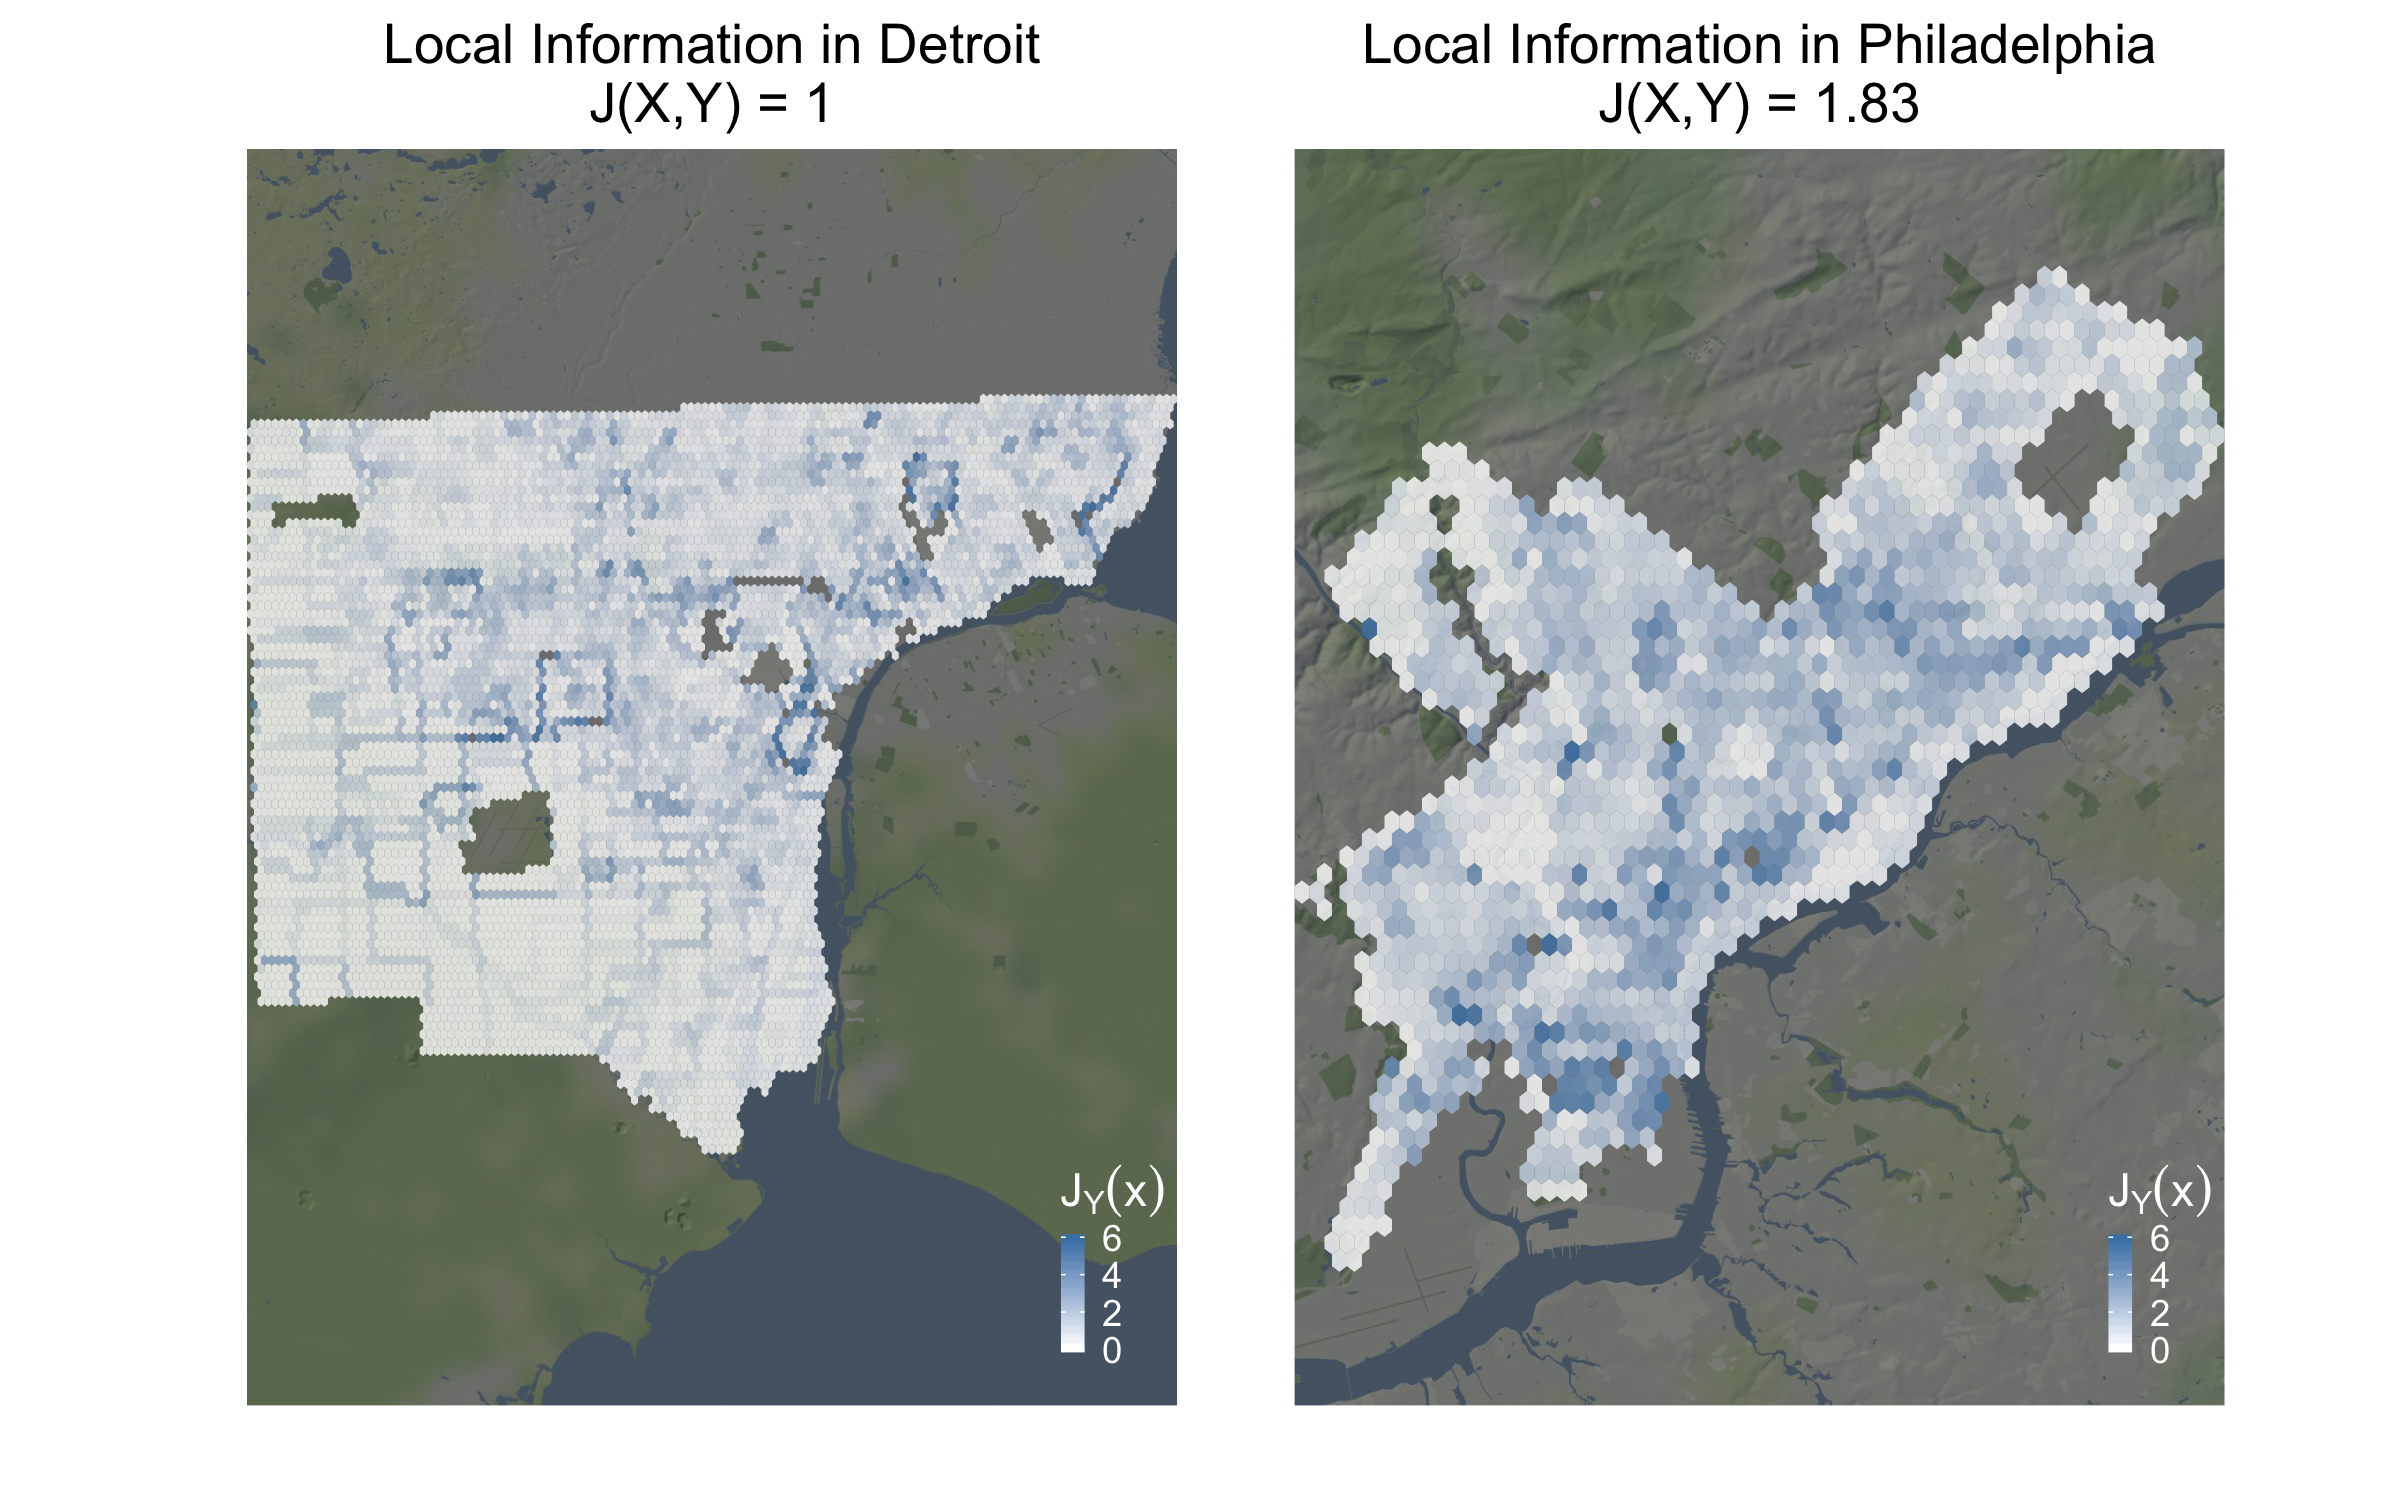
\includegraphics[width=.8\textwidth]{figs/method_illustration.png}
		\caption{Illustration of methodology for estimating local information in Suffolk County, MA (Boston). We first cover the map in a hexgrid, and compute the mutual information within each hex from the Census tracts that overlap the hex, weighted by density. }
		\label{fig:method}
	\end{figure}


	Figure \ref{fig:info_cross} shows the relationship of the mutual information (or evenness) $I(X,Y)$ and mean local information (or exposure) $J(X,Y)$. The global positive trend reflects the fact that global spatial variability is a prerequisite for local variability: if the city is uniform (like Figure \ref{fig:toy}(a)), then no local differences either exist.  On the other hand, there are substantial variations in $J(X,Y)$ even in cities with comparable global variability $I(X,Y)$. For example, the cities of Detroit and Philadelphia provide a striking contrast. While they have mutual information $I(X,Y)$, Philadelphia's mean local information $J(X,Y)$ is substantially higher. This reflects the fact that Detroit is composed of large, highly-segregated, monoracial neighborhoods, whereas Philadelphia has a much more fine-grained, intricate neighborhood structure. These patterns illustrate how combinations of the information measures $H(Y)$, $I(X,Y)$, and $J(X,Y)$ can be used to construct taxonomies diversity for American cities. It may be useful summarise the two measures by calling cities close to the bottom-right ``most segregated'', but we recommend reporting both $I(X,Y)$ and $J(X,Y)$. It is best to compare $J(X,Y)$ only between cities with similar $I(X,Y)$; thus, while it may be right to say that Detroit has lower levels of exposure than Phildelphia, when comparing Detroit to Baltimore it should be kept in mind that Baltimore is more even in its overall sociospatial structure. 
	\begin{figure}
		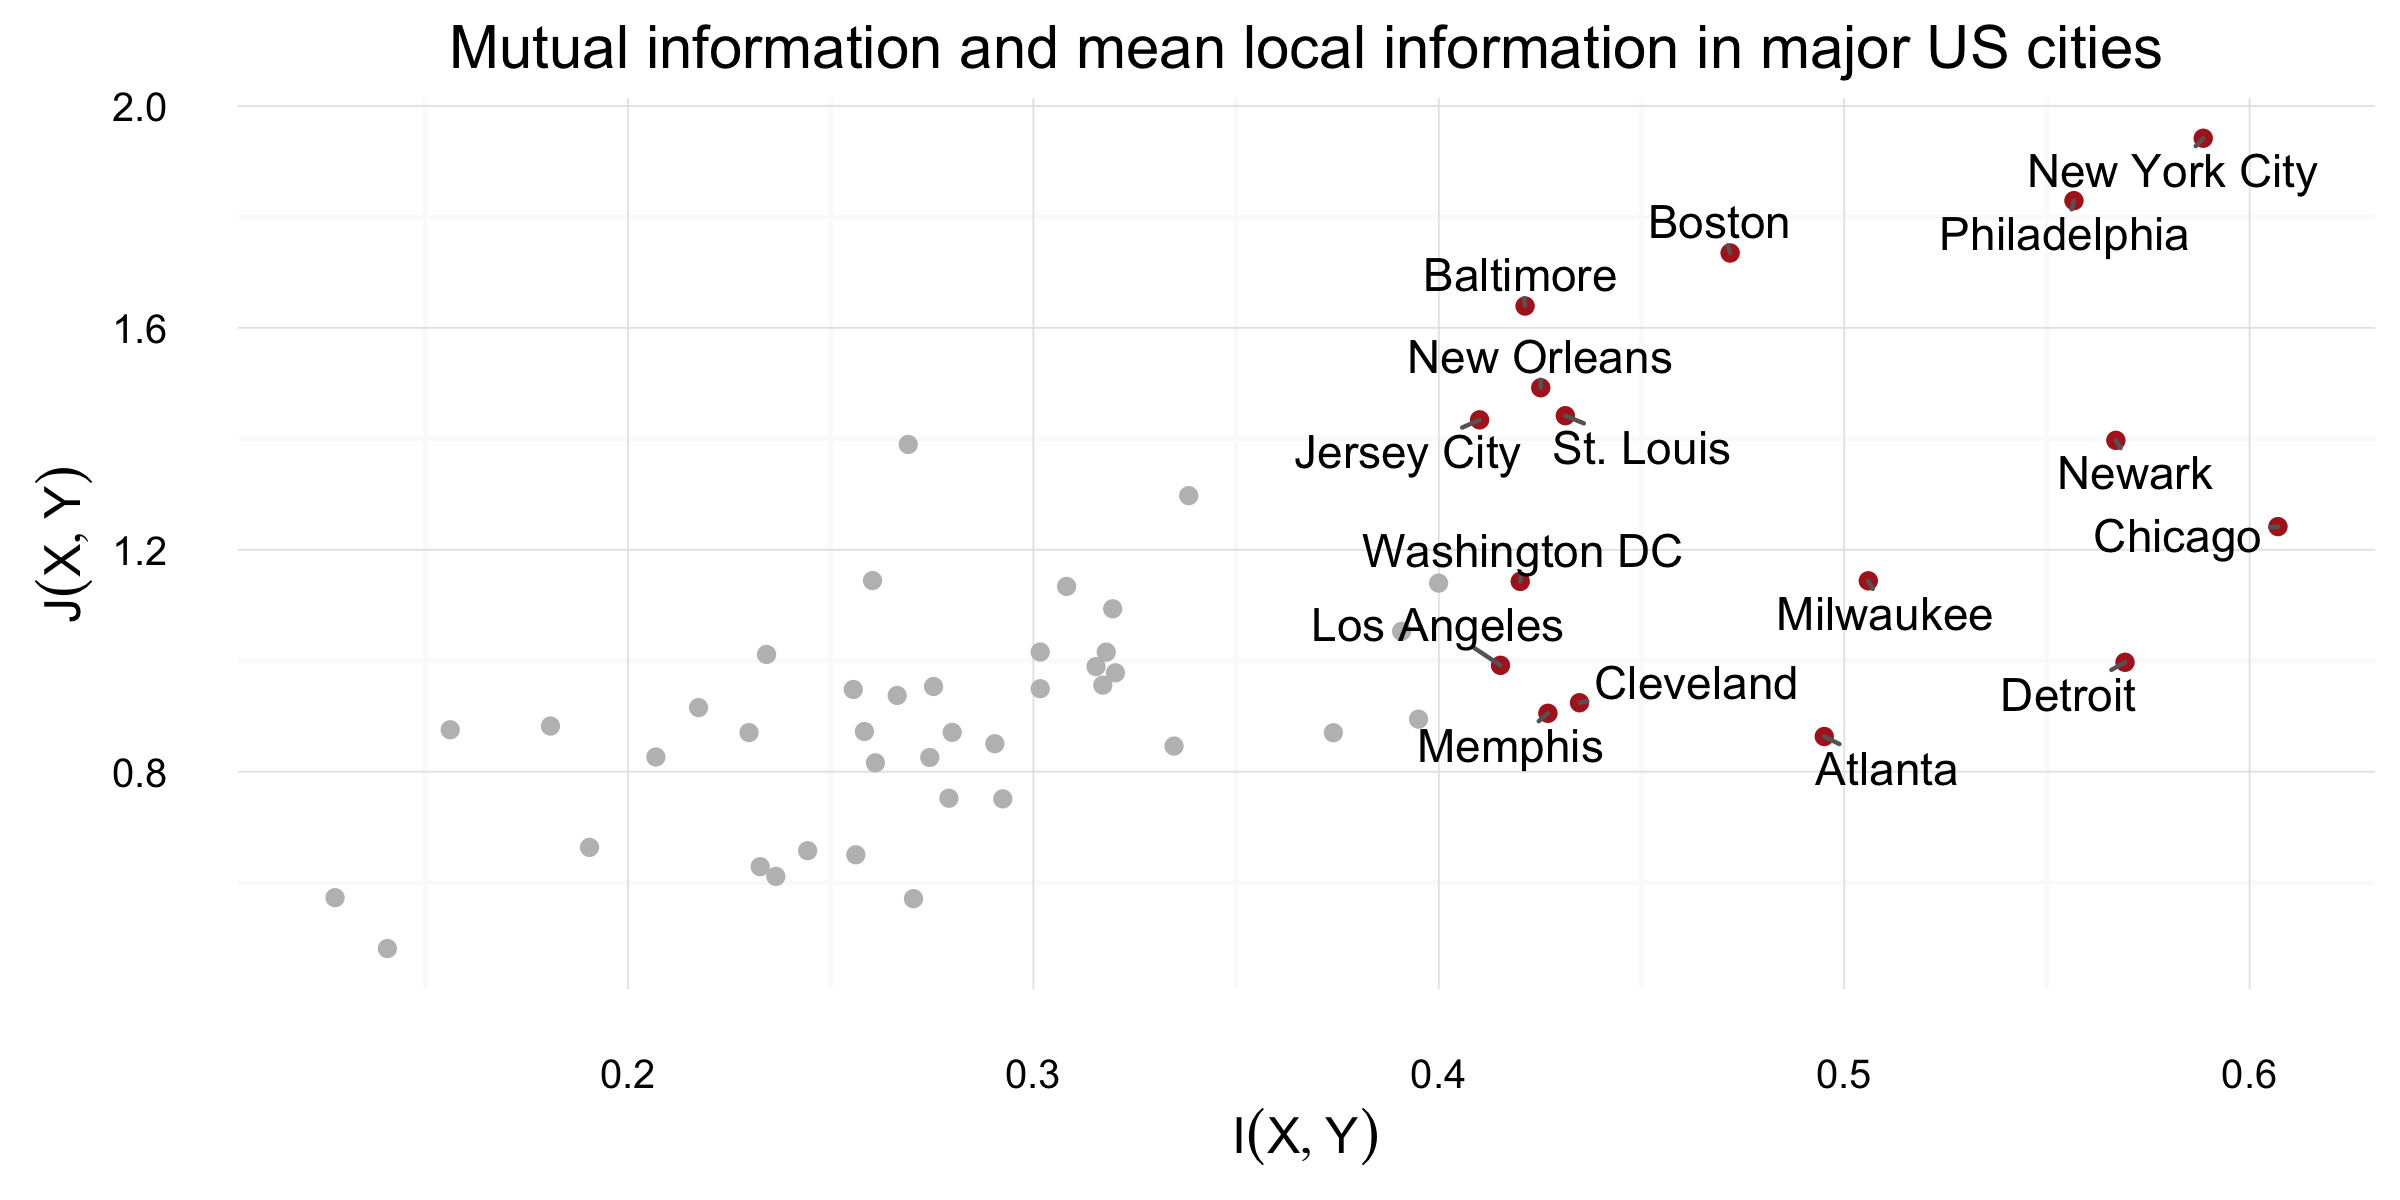
\includegraphics[width=1\textwidth]{figs/mutual_fisher.png}
		\caption{Relationship of global mutual information $I(X,Y)$ and mean local information $J(X,Y)$.} 
		\label{fig:info_cross}
	\end{figure}	


	
	\begin{figure}
		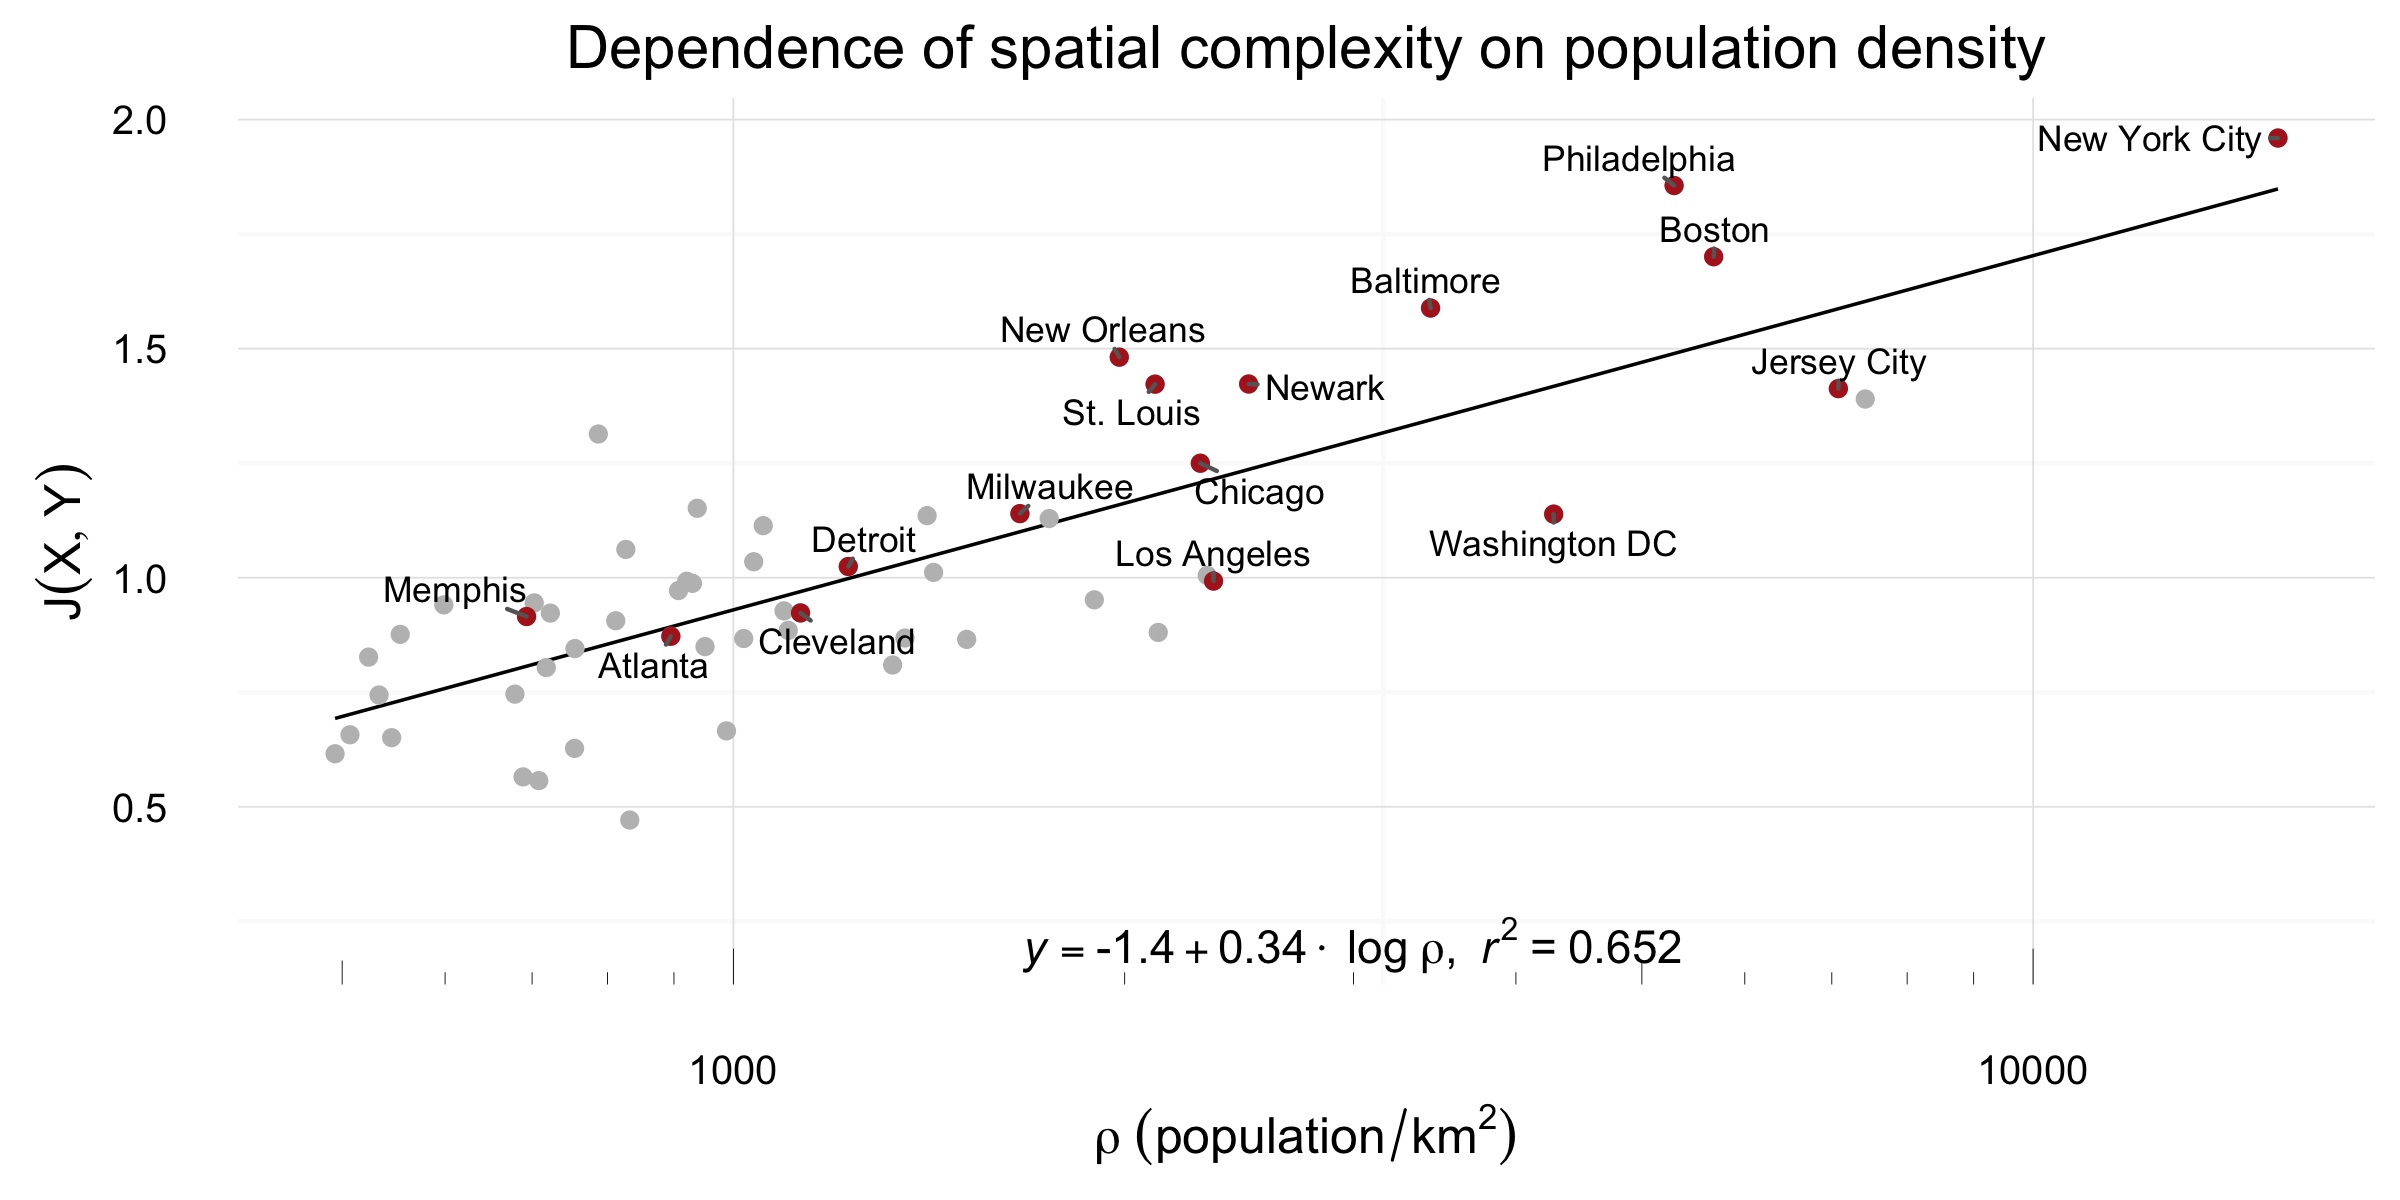
\includegraphics[width=1\textwidth]{figs/density_fisher.png}
		\caption{The mean local information $J(X,Y)$ scales with the logarithm of population density.}
		\label{fig:density}
	\end{figure}	

	Intriguingly, the mean local variability $J(X,Y)$ appears obey a scaling relation with respect to urban density. In Figure \ref{fig:density}, we plot $J(X,Y)$ against the population density $\rho$ of our studied cities. It appears that $J(X,Y)$ grows linearly with the logarithm of density. We interpret this trend as reflecting a compression of social space in dense urban areas: the same structure of racial variability fits into much less geographical area in New York than in Phoenix. One aspect of diversity in large, dense cities is that one need walk much less distance in order to reach a neighborhood with substantially different racial trends than one's own. It may be of interest for later studies to consider why this trend might arise through dynamical processes of urban formation. 
	 
\subsection*{Learning From Natural Neighborhoods}

	Figure \ref{fig:cluster_map} shows an illustrative clustering of Wayne County (housing the city of Detroit) into six regions using the greedy information maximization procedure defined by equation \eqref{eq:info_dist}. The procedure cleanly divides the city into racially coherent zones. Cluster A is predominantly white and B predominantly black, demarcating the major racial divide in the city. Cluster C is a small transitional zone in which the two races overlap. Clusters D and E are the demographically distinct independent cities of Hamtramck and Grosse Pointe, respectively, while Cluster F is a Hispanic community known as Mexicantown. The existence of clusters like C reflects that not every racially coherent tract is interpretable as a ``neighborhood''; some may be more naturally thought as transitions between neighborhoods. 
	
	\begin{figure}
		\centering
		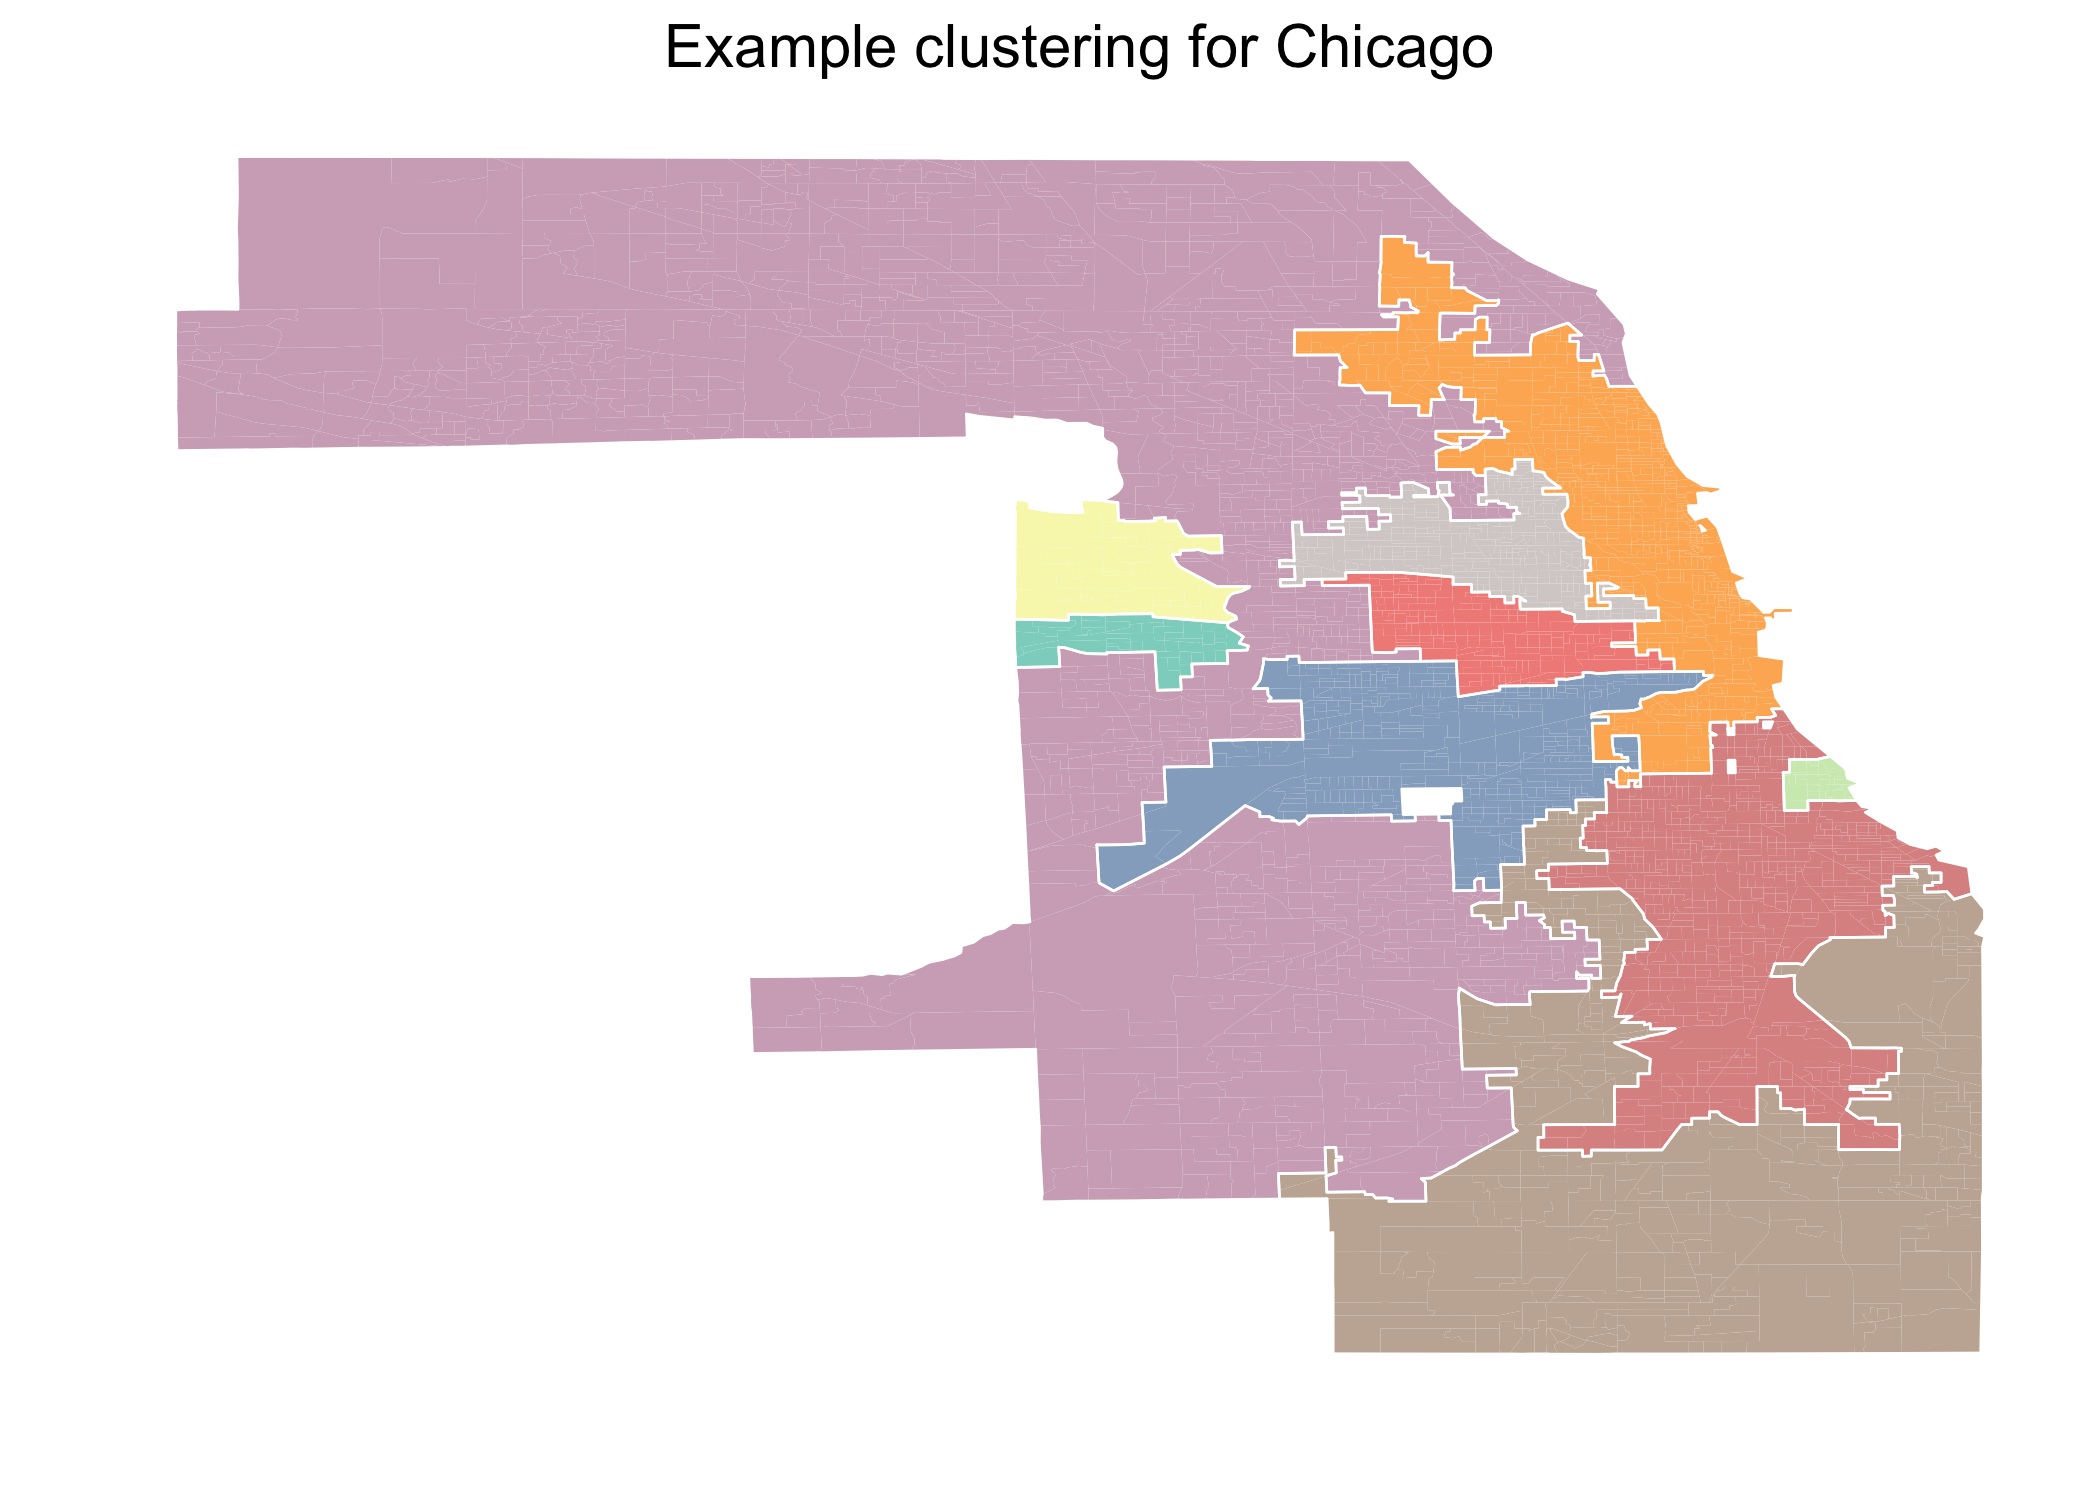
\includegraphics[width=\textwidth]{figs/example_cluster_map.png}
		\caption{Clustering of Detroit into 6 neighborhoods based on race.}
		\label{fig:cluster_map}
	\end{figure}		

	Cities vary sharply in the level of cluster detail needed to convey equal amounts of demographic information. Figure \ref{fig:clusters} shows example cluster divisions for four major cities. Each clustering conveys approximately equal demographic information, as measured by the mutual information $I(C,Y)$ between cluster labels and racial distribution. In sharply segregated Atlanta, just two clusters--one predominantly white, the other predominantly black--suffice to convey as much information as five in Boston, where the clusters are substantially more nuanced. Boston's Cluster A is predominantly white, cluster D majority Hispanic, and cluster E majority black. Cluster B is again majority white, but is distinct in that its minority citizens are almost all Hispanic. Cluster C is approximately equally black, Hispanic, and white. 

	Clusterings such as those shown in Figure \ref{fig:clusters} shed useful light on traditional concerns in the study of segregation. We have already argued that $I(X,Y)$ and $J(X,Y)$ naturally encode the high-level ideas of evenness and exposure endorsed by \cite{Reardon2004}. We now consider the further concepts of clustering and concentration. According to \cite{Massey1988}, ``\emph{clustering} measures the degree to which minority areas are located adjacent to one another'' and ``\emph{concentration} refers to the degree of a group's agglomeration in urban space'' (pages 309-310). When areas with similar racial composition are located close to one another, fewer spatial clusters are necessary to convey equivalent information about racial trends. Thus, \ref{fig:clusters} suggests that Atlanta is more clustered than Boston, a suggestion that we can quantify using the AUC methodology developed below. The concept of concentration invites us to consider the composition and density of each cluster. In Detroit, for example, whites make up 70\% of ``their'' Cluster A, while black residents make up a full 86\% of ``their'' Cluster B. Cluster B is also more concentrated in that it is more densely populated than Cluster A: it contains 34\% of the Detroit's population, but accounts for just 19\% of land in the analyzed area. This makes Cluster B more than twice as dense as Cluster A. Thus, in Detroit, ``black'' neighborhoods tend to be more racially homogeneous and more densely packed in urban space than ``white'' ones. Finally, we note that these clusterings allow us to examine the somewhat abstract concept of ``exposure'' in considerable detail. Figure \ref{fig:clusters} indicates that across all cities, Asians are much more likely to be found in predominantly white clusters than they are in predominantly black or Hispanic ones, indicating significant spatial integration between these two groups. In Chicago, some groups of Hispanics are exposed primarily to Hispanics and other whites (Cluster B), while other groups are exposed primarily to black residents (Cluster D).

	\begin{figure}
		\centering
		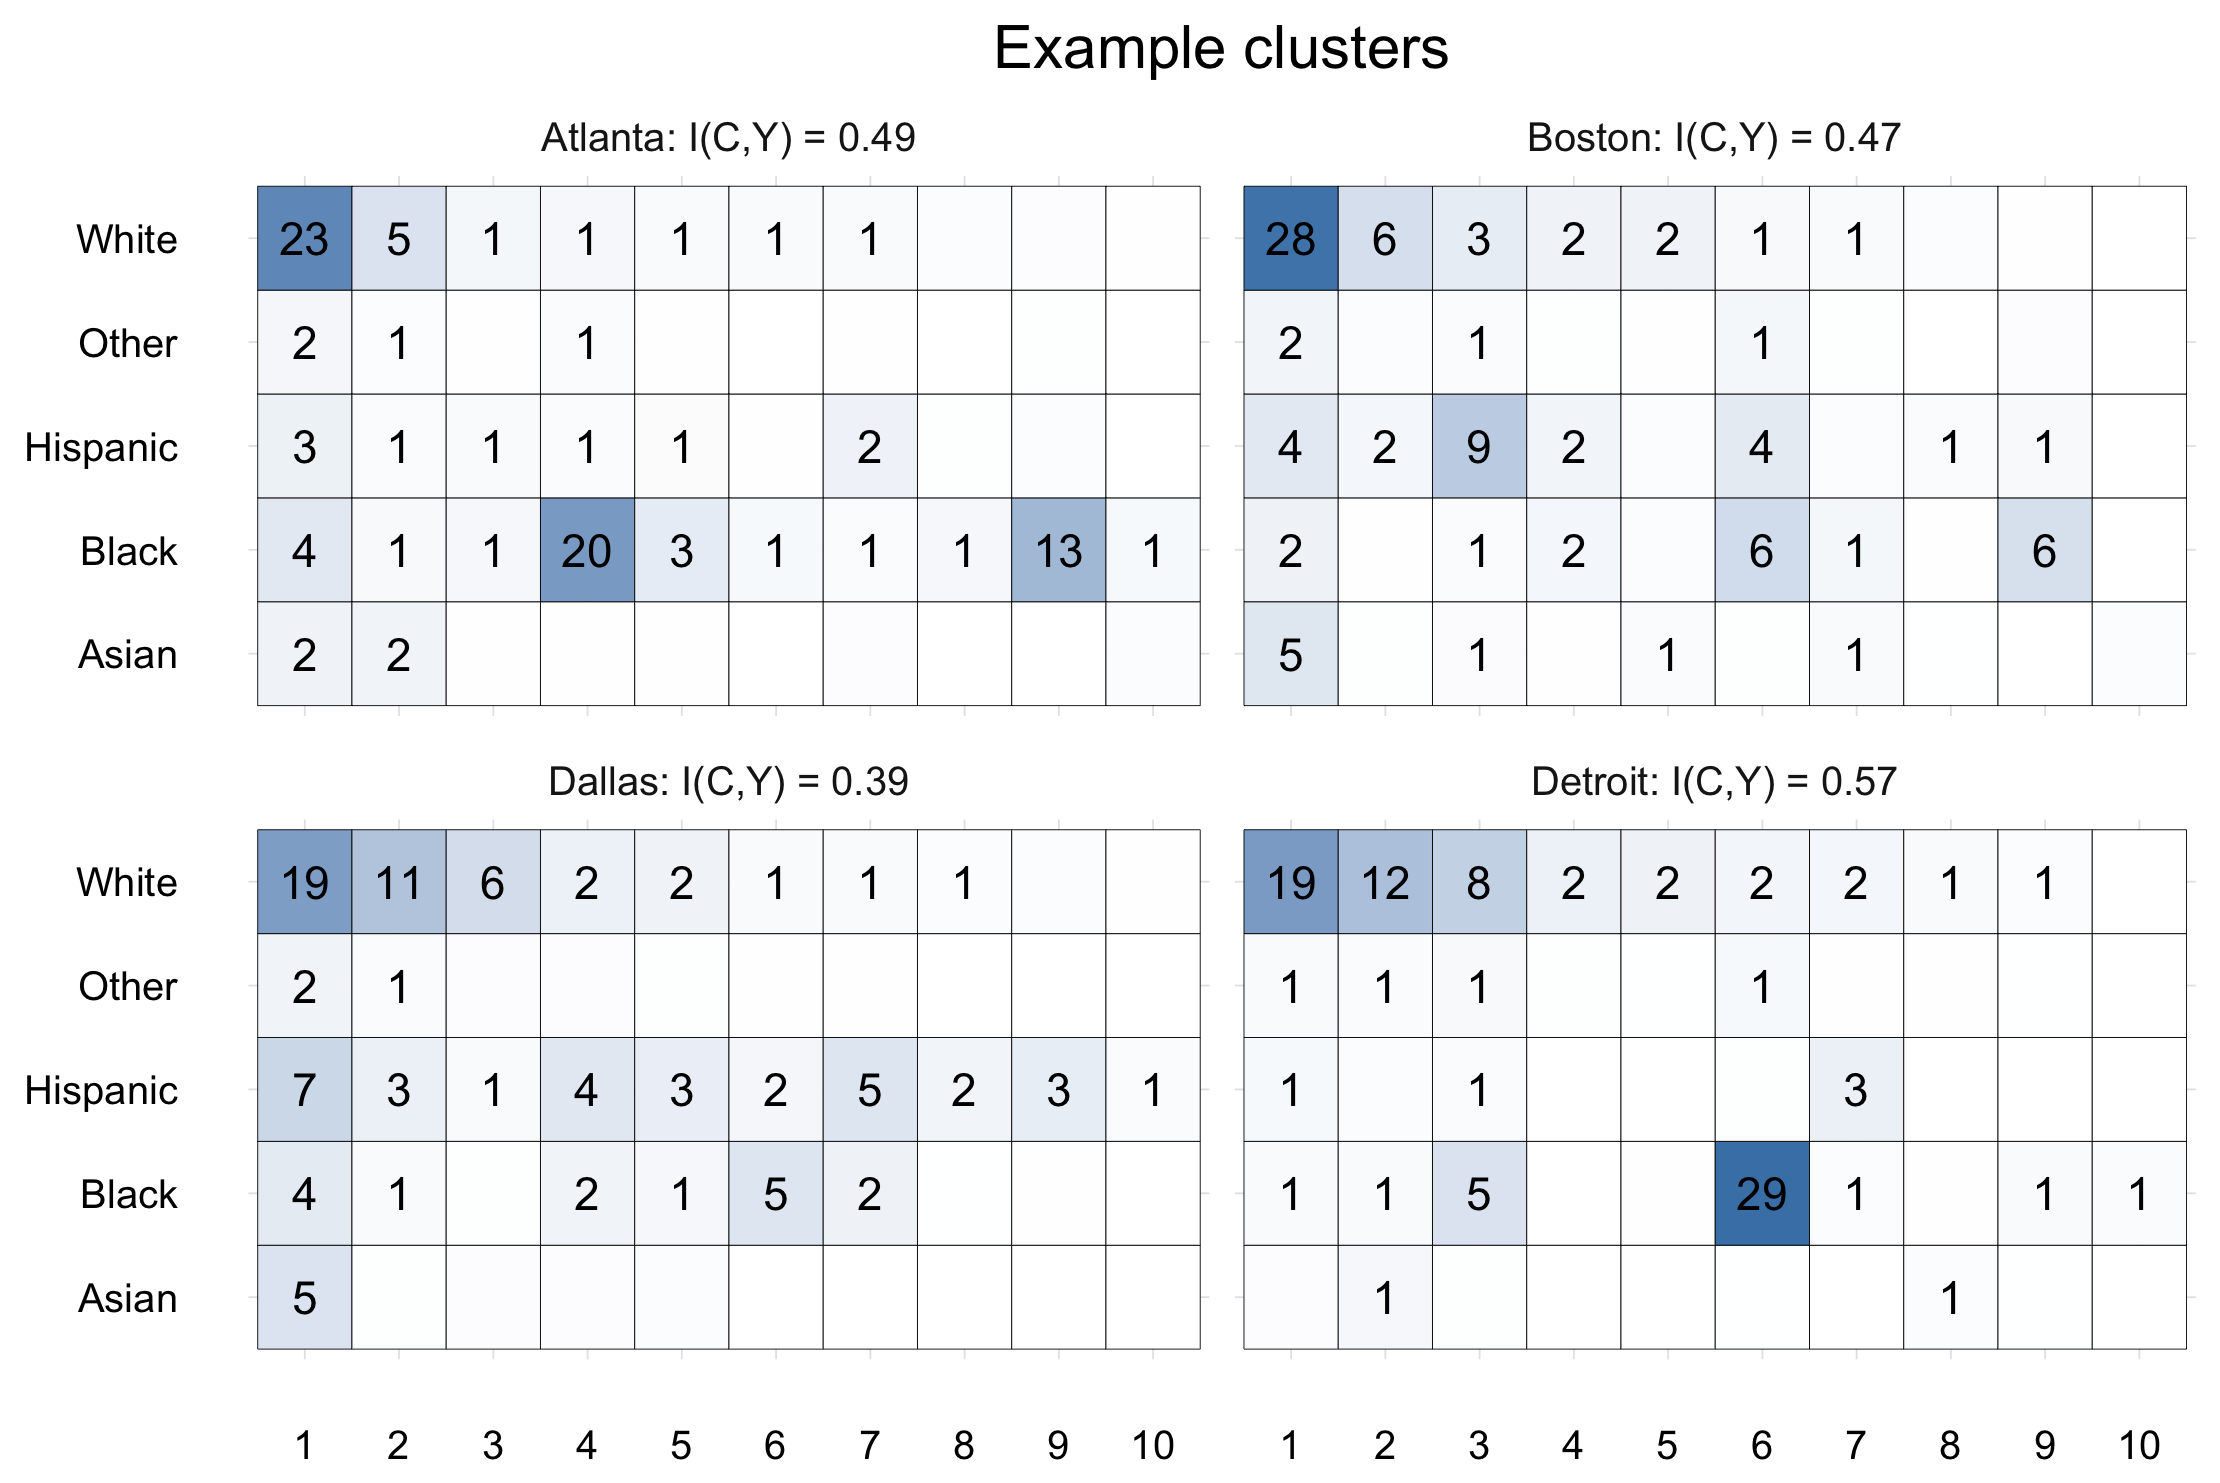
\includegraphics[width=\textwidth]{figs/example_clusters.png}
		\caption{Example clusters for different cities, and the associated mutual information contained in each. The number in each box reflects the percentage of the population in the labeled racial group and cluster. }
		\label{fig:clusters}
	\end{figure}

\subsection*{Complexity and Neighborhood Structure}

	We expect that spatially complex cities with high $J(X,Y)$ would require more complicated models in order to capture similar levels of spatiosocial structure. Testing this expectation requires a quality measure defined on cluster models for each city. The natural measure of loss for a clustering is the mutual information $I(C,Y)$ between cluster and racial labels.
		
	To develop a global evaluation of the hierarchical clustering of a city according to the method defined by \eqref{eq:info_dist}, we borrow the methodology of the ``area under the curve'' (AUC) used extensively in statistical learning. By plotting the information $I(C,Y)$ against the number of clusters $n$, we obtain a curve reflecting how the information evolves at varying scales of aggregation. Figure \ref{fig:AUC} illustrates these curves for Boston and Detroit, with $N$ plotted on a logarithmic scale.  

	\begin{figure}
		\centering
		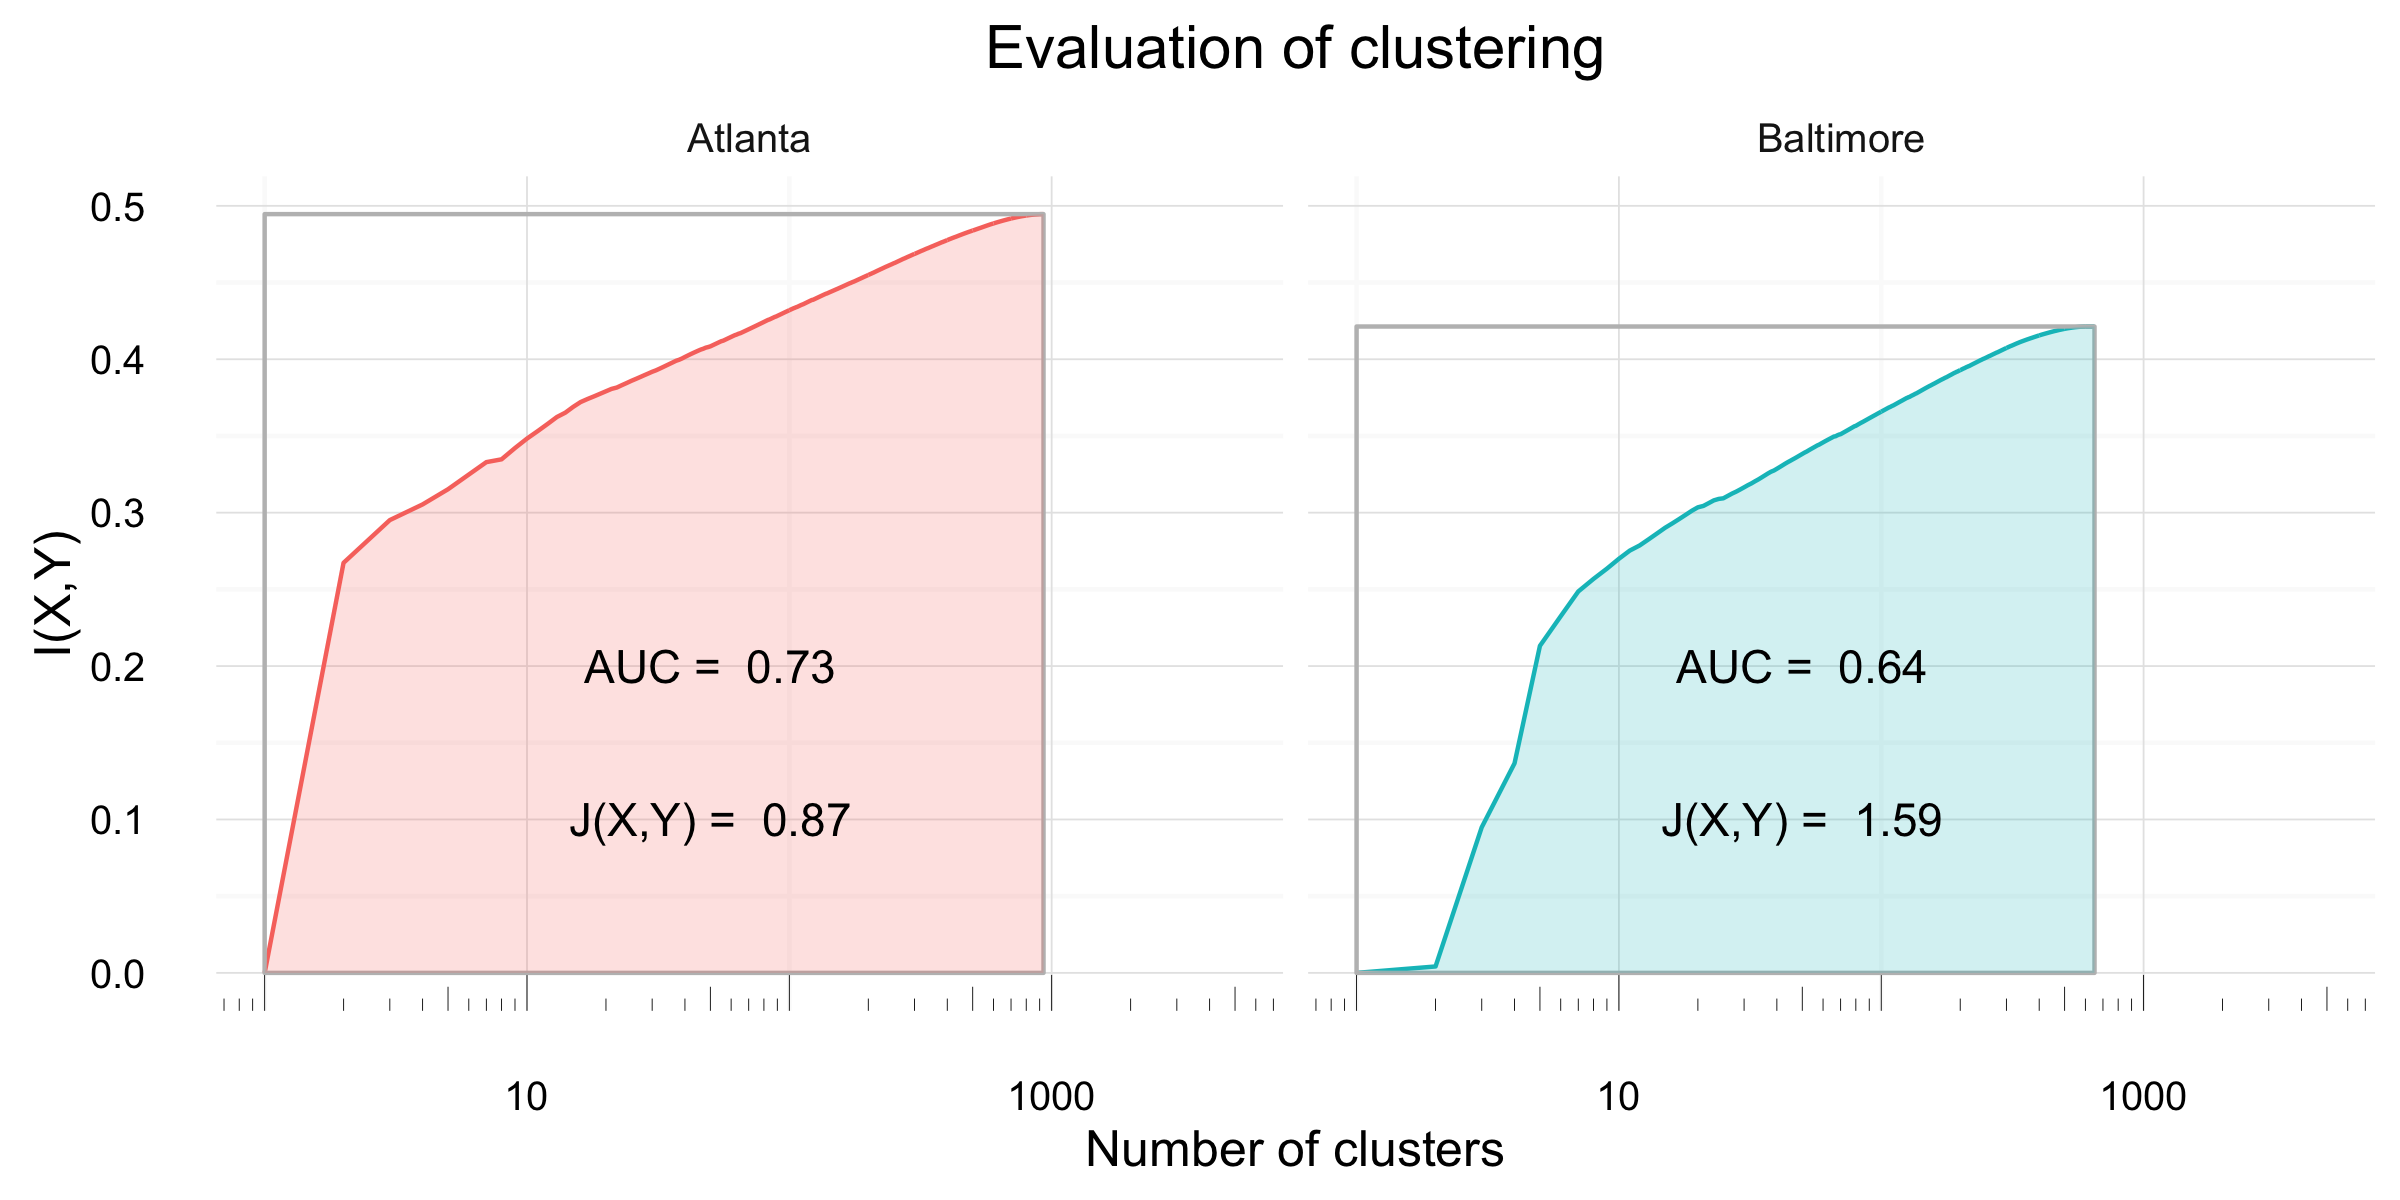
\includegraphics[width=\textwidth]{figs/AUC_illustration.png}
		\caption{Evaluation of clustering using an Area Under the Curve (AUC) metric. The AUC is the fraction of the bounding box lying under the information gain curve. Boston's AUC is smaller than Detroit's, showing that Boston's spatial complexity (measured by $J(X,Y)$) requires more complex models than Detroit's.}
		\label{fig:AUC}
	\end{figure}

	Figure \ref{fig:AUC} also shows the bounding rectangle, whose top right corner is defined by the number N of tracts in the census data set and the full mutual information $I(X,Y)$. The AUC is defined as the ratio of the shaded area in Figure \ref{fig:AUC} to the bounding rectangle, and is computed via the formula 

	\begin{equation}
		A = \frac{1}{I(X,Y) \log N }\sum_{n = 1}^N I(C_n, Y) \log \frac{n + 1}{n}  ,
	\end{equation}

	where $N$ is the total number of Census blockgroups and $C_n$ is the cluster label at the level in which $n$ total clusters are defined.

	When $A = 1$, it must hold that $I(C_1,Y) = I(X,Y)$. This implies that just one region carries full information; this can only occur in a city with no spatial unevenness, such as city (b) in \ref{fig:toy}. More generally, a large AUC indicates that simple models with few distinct regions capture much of the information about spatial variation in the city. In Atlanta, there exists a clear dividing line between a predominantly white region in the north and a predominantly black region in the south. A two-cluster model therefore captures much of the information in the city, giving a high AUC of 0.71. In Boston, on the other hand, no such clear divide exists, and more complex models are necessary to capture similar amounts of information. Thus, Boston has a lower AUC of 0.65. 

	\begin{figure}
		\centering
		% 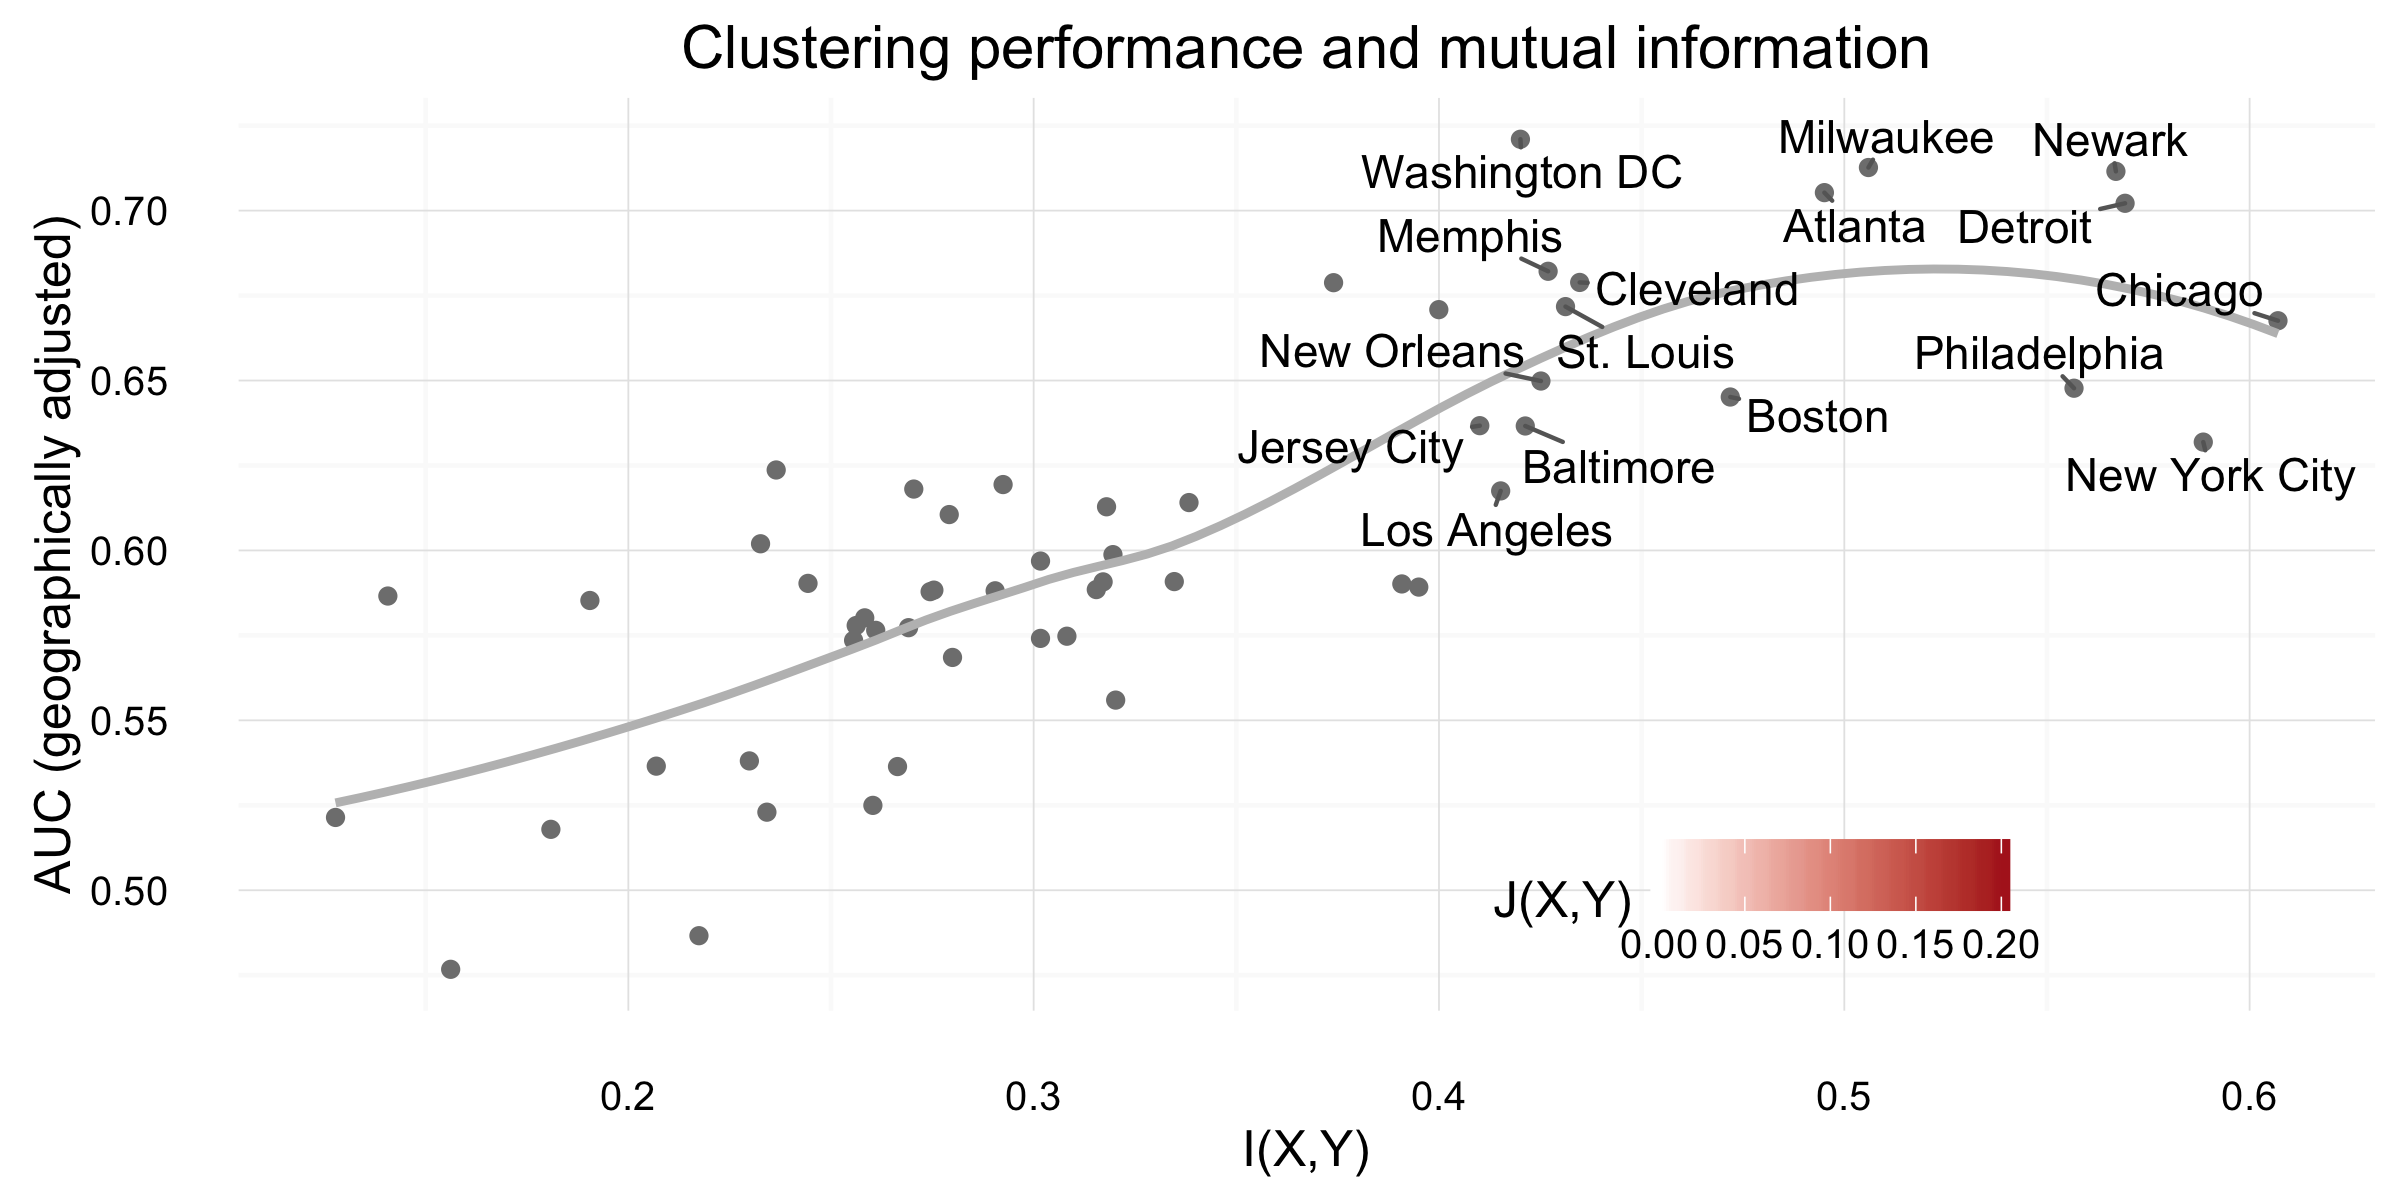
\includegraphics[width=\textwidth]{figs/info_performance_adjed.png}
		\input{figs/adjusted_regression.txt}

		\caption{Summary of regression of the clustering AUC on information measures $H(Y)$, $I(X,Y)$, $J(X,Y)$. The AUC has been geographically adjusted to account for cities like New York, whose Census blockgroups form eight disconnected components, which would mildly distort results without adjustment. Table produced using \cite{Marek2015}}.
		\label{fig:info_and_clusters}
	\end{figure}		

	We argued previously that $H(Y)$, $I(X,Y)$, and $J(X,Y)$ provide a multi-dimensional characterization of spatial diversity in a city. Based on this discussion, we would expect that the performance of our clustering algorithm, as measured by the AUC, is closely related to these measures. Figure \ref{fig:info_and_clusters} confirms this expectation using simple linear regression of the AUC on the three measures. Overall, these three information measures explain approximately an adjusted 75\% of the ``clusterability'' of cities. The signs associated with $I(X,Y)$ and $J(X,Y)$are suggestive: it is easiest to identify natural neighborhoods when there is substantial spatial variation (high $I(X,Y)$) but relatively simple local structure (low $J(X,Y)$). 